% !TEX TS-program = lualatex
% !TEX encoding = UTF-8 Unicode

\documentclass[]{einformatica}
\usepackage{graphicx}
\usepackage{soul}
\usepackage{booktabs}
\usepackage{hyphenat}
\usepackage[all]{nowidow}
\usepackage{tabularx} 
\usepackage{floatrow} 
\floatsetup[table]{style=plain,capposition=top}
\renewcommand\topfraction{.95}
\renewcommand{\textfraction}{0.05}
\usepackage{refcount} 
\usepackage[noadjust]{cite} 

\usepackage{xcolor}
\usepackage{hyperref}
\hypersetup{
    urlbordercolor = black,
    pdfborderstyle={/S/U/W 1},
}

\usepackage[newfloat]{minted}
\setminted[R]{breaklines=true,fontsize=\footnotesize,obeytabs=true,tabsize=0}
\setmintedinline[R]{breaklines=true,fontsize=\footnotesize}

\usepackage{listings}
\newenvironment{code}{\captionsetup{type=listing}}{}
\SetupFloatingEnvironment{listing}{name=Listing}

\usepackage[resetlabels,labeled]{multibib}

\usepackage{tikz}
\usetikzlibrary{shapes.geometric, arrows.meta, positioning, fit, backgrounds}
\usepackage{pgfplots}
\pgfplotsset{compat=1.18}
\usepackage{subcaption}

 \begin{document}

\title{Proactive Multimodal Academic Support System: A Smart Campus Initiative}

\shortauthorshead{Usha Vemireddy et al.}

\eIsubmitted{} 
\eIrevised{-} 
\eIaccepted{-}
\eIpublished{-} 

\EIauthorII
   {Hari}
   {Battana}
   {Assistance Professor, Malla Reddy University}
   {battana\_hari@mallareddyuniveristy.ac.in}
   {0009-0004-8005-7871} % ORCiD ID
   {} %  if star present means corresponding author


\EIauthorIV
   {Subhapreet}
   {Patro}
   {Department of Computer Science Engineering \\ Malla Reddy University, India}
   {subhapreetpatro2004@gmail.com}
   {0009-0004-1274-7248} % ORCiD ID
   {} %  if star present means corresponding author

\EIauthorIII
   {Sreeja}
   {Uplanchiwar}
   {Department of Computer Science Engineering \\ Malla Reddy University, India}
   {sreejauplanchiwar721@gmail.com}
   {0009-0004-9686-3368} % ORCiD ID
   {} %  if star present means corresponding author

\EIauthorI
   {Usha}
   {Vemireddy}
   {Department of Computer Science Engineering \\ Malla Reddy University, India}
   {ushareddyvemireddy@gmail.com}
   {0009-0001-2669-9361} % ORCiD ID
   {*} %  if star present means corresponding author

\EIauthorV
   {Bhavana}
   {Yelagandala}
   {Department of Computer Science Engineering \\ Malla Reddy University, India}
   {bhavanayelagandala@gmail.com}
   {0009-0001-4807-9497} % ORCiD ID
   {} %  if star present means corresponding author
   
 \keywordset{Proactive System, Multimodal Interaction, Academic Support, Artificial Intelligence, Smart Campus, Mobile Computing, Software Engineering} 

\begin{abstract}[en] 
\textbf{Context}:
The education sector is undergoing a massive digital transformation. However, existing university stakeholder interactions remain fragmented across legacy web portals, physical notice boards, and disparate communication threads, leading to administrative inefficiencies and a disjointed user experience. \\ 
\textbf{Objective}: 
This study presents the design, implementation, and empirical evaluation of a "Smart Campus" system named the Proactive Multimodal Academic Support System (PMASS). The goal is to provide a cohesive, proactive, and intelligent ecosystem that modernizes institutional infrastructure through Artificial Intelligence and optimized data delivery. \\
\textbf{Method}: 
A Service-Oriented Architecture (SOA) was implemented, featuring a cross-platform Flutter mobile client, a Node.js API gateway, and a Supabase (PostgreSQL) data layer. The system integrates Google Gemini AI for Retrieval-Augmented Generation (RAG) and predictive attendance analytics via a specialized Stale-While-Revalidate (SWR) caching strategy. \\
\textbf{Results}: 
Empirical evaluation through a four-week pilot study ($n=48$) demonstrates significant improvements in campus accessibility and administrative efficiency. The system achieved a 90\% reduction in information-retrieval latency compared to legacy portals, with a mean System Usability Scale (SUS) score of 81.4. Performance benchmarks confirm sub-100ms dashboard latency enabled by the SWR architecture. \\
\textbf{Conclusions}: 
The PMASS successfully bridges communication gaps and reduces administrative overhead. By shifting from reactive data silos to proactive AI-driven analytics, the platform serves as a validated architectural blueprint for digital-first educational institutions.
\end{abstract}

\maketitle 
 

\section{Introduction}\label{sec:Introduction}

The education sector is currently experiencing a rapid and necessary shift towards comprehensive digital transformation. Traditional administrative processes and fragmented digital tools are progressively being replaced by integrated smart campus solutions. This paper presents the Proactive Multimodal Academic Support System (PMASS), a pioneering initiative designed to fundamentally modernize the university experience. It achieves this by leveraging the latest advancements in Mobile Computing, Cloud Infrastructure, and Generative Artificial Intelligence (AI), while providing a rigorous empirical evaluation of its operational efficacy. 

In a typical university setting, stakeholders—including students, faculty, and administrators—often operate in isolated silos. Critical information is frequently fragmented across physical notice boards, legacy web portals, disparate email threads, and informal social media groups. This fragmentation inevitably results in communication silos, administrative inefficiencies, and an overall disjointed user experience that fails to meet the expectations of modern digital-native students.

\subsection*{Problem statement} 

Despite the growing availability of various digital tools in educational institutions, the academic environment faces critical and persistent challenges. Information asymmetry consistently leads to students missing vital updates, such as sudden changes in exam schedules or venue relocations, primarily because these notices are not pushed in real-time. Additionally, administrative offices are frequently overwhelmed by students presenting redundant queries regarding syllabus verifications, lab timings, or standard administrative procedures, causing significant bottlenecks. 

Furthermore, the lack of interactive navigation tools makes physical campus traversal confusing for newcomers and visitors, who must rely on static 2D maps lacking contextual guidance. Finally, traditional attendance systems remain purely reactive ledgers. They fail to proactively identify students at risk of falling behind until the end of the semester, leaving faculty without the timely analytics needed to intervene effectively.

\subsection*{Research objective}

The primary objective of this research is to design, develop, and evaluate a single, unified robust mobile platform that aggregates all academic, administrative, and co-curricular information. Specific technological objectives include:
\begin{itemize}
    \item Deploying a context-aware AI-powered assistant capable of Natural Language Understanding (NLU) to serve as a first-line responder for student queries via Retrieval-Augmented Generation (RAG).
    \item Utilizing immersive 3D technology to provide a virtual tour for seamless campus navigation, accompanied by scene-specific AI guidance.
    \item Shifting towards proactive analytics by generating automated, predictive attendance trend forecasts and automated student performance insights safely synced across a cloud architecture.
\end{itemize}

\subsection*{Study context}

The study takes place in the context of modern university campuses seeking to align with Industry 4.0 standards. As institutions expand both physically and demographically, upgrading their digital infrastructure to support automated, asynchronous communication and intelligent resource management becomes imperative.

\subsection*{Contribution statement}

This paper contributes a comprehensive system architecture and practical implementation of a unified digital ecosystem. It successfully demonstrates the merging of strict Role-Based Access Control (RBAC) \cite{sandhu1996}, real-time data synchronization via WebSockets, and distributed load-balancing for Generative AI (RAG) to form a robust, proactive smart campus solution.


\section{Background}\label{sec:Background}

The integration of artificial intelligence in educational environments has paved the way for more sophisticated support mechanisms that extend beyond mere digitization \cite{yang2023, li2023}. Legacy Learning Management Systems (LMS) historically prioritize course content delivery and assignment tracking, while static university websites serve strictly as passive information repositories. 

Modern educational challenges require a "Digital First" approach where technology actively nudges students toward academic success. This operational paradigm shift focuses on multimodal interaction—combining natural language text processing, voice, and interactive visual 3D navigation. By anticipating user needs, such as automatically displaying the next scheduled class or directly answering policy queries based on the university's official handbook, multimodal interfaces prove highly effective at reducing cognitive load for both students and staff.

\section{Related Work}\label{sec:RelatedWork}

A comprehensive review of existing educational platforms reveals a distinct gap in holistic campus life integration \cite{amershi2023, yao2023}. Traditional platforms such as Google Classroom excel at assignment distribution but lack real-time administrative synchronization and broader campus utility. Established LMS platforms like Moodle require extensive custom plugin configurations for basic AI capabilities and frequently suffer from generic, non-native mobile web-view experiences.

Recent work by Gao et al.~\cite{gao2024rag} provides a comprehensive taxonomy of Retrieval-Augmented Generation (RAG) architectures and demonstrates their superiority over parametric-only language models for domain-specific question-answering—directly motivating our integration of a pgvector-based RAG pipeline. Hwang and Tu~\cite{hwang2024smartcampus} conducted a systematic review of Smart Campus research trends between 2015 and 2024, identifying three unmet integration gaps: unified role-based access, proactive student risk notification, and immersive spatial navigation. All three gaps are directly addressed by the proposed system. Concurrent benchmarking work by Chen et al.~\cite{chen2024llmeval} evaluating large language models in RAG settings confirms that retrieval quality—particularly chunk granularity and embedding model selection—is the single largest determinant of answer faithfulness, informing our choice of \texttt{gemini-embedding-001} for the knowledge base.

Similarly, standard university web portals lack role-based personalization—presenting the same static interface to a first-year student as they do to a department head—and rely solely on elementary 2D maps for spatial navigation. The proposed system deliberately fills these identified gaps by providing high real-time responsiveness through native mobile rendering (Flutter), an integrated Google Gemini RAG AI, a 360-degree virtual tour featuring gyroscopic capability, and role-specific dynamic dashboards customized for students, faculty, and administrators.

\begin{table*}[htbp]
\centering
\caption{Comparison of the Proposed System versus Existing Educational Platforms}
\label{tab:platform_comparison}
\resizebox{\textwidth}{!}{%
\begin{tabular}{@{}lcccc@{}}
\toprule
\textbf{Feature} & \textbf{Google Classroom} & \textbf{Moodle (LMS)} & \textbf{Static Web Portals} & \textbf{Proposed System (Campus Assistant)} \\ \midrule
Primary Focus & Assignment/Content & Course Management & Information Repository & \textbf{Holistic Campus Life} \\
Real-Time Updates & Moderate (Email) & Low & Low & \textbf{High (WebSockets)} \\
AI Assistance & None & Requires Custom Plugin & None & \textbf{Integrated Gemini RAG} \\
Campus Navigation & None & None & 2D Static Maps & \textbf{360-degree Virtual Tour} \\
Mobile UX & Excellent & Generic Web-view & Poor & \textbf{Native Flutter (60FPS)} \\
Personalization & Class-based & Course-based & None & \textbf{Strict Role \& Context-based} \\ \bottomrule
\end{tabular}%
}
\end{table*}

\section{System Design and Implementation}\label{sec:Method}

\subsection*{Research goal and hypotheses}

The core research goal evaluates whether a proactive, AI-driven multimodal interface can significantly reduce administrative overhead and improve the precise accessibility of campus information compared to traditional distinct platforms. We hypothesize that integrating context-aware AI directly into operational academic workflows will lower redundant query volumes by at least 40\% and increase timely intervention for at-risk students.

\subsection*{Research method / procedure}

The project adopted an Agile Software Development Life Cycle (SDLC) with iterative 2-week development sprints, incorporating continuous integration. The system design relies on a highly decoupled Service-Oriented Architecture (SOA). 

\textbf{Frontend Architecture:} The client layer utilizes the Flutter (Dart) framework, guaranteeing native performance across iOS and Android ecosystems with a 60FPS glassmorphic user interface. Critical data such as timetables and the user's latest AI forecasts are persistently cached locally using Hive, ensuring strict offline-first reliability.

\textbf{Backend and Data Layer:} The gateway layer operates on Node.js (TypeScript) running Express, handling authentication middleware, rate limiting, and business logic routing. All relational data, vector embeddings for AI similarity searches, and object storage are managed securely via Supabase (PostgreSQL 15 paired with the \texttt{pgvector} extension). Strict row-level security (RLS) policies enforce data isolation based on JWT session tokens \cite{supabase2024, owasp2023}.

\textbf{Artificial Intelligence Infrastructure:} The AI capabilities run on the Google Gemini API (utilizing \texttt{gemini-2.5-flash} for generation and \texttt{gemini-embedding-001} for vectorization) \cite{gemini2024, openai2024}. To guarantee high system reliability and bypass strict rate limits, the backend implements a distributed round-robin key rotation load balancer managing multiple concurrent API keys.

For attendance and performance tracking, a highly optimized AI insight engine was developed that formalizes two algorithms from the backend implementation. First, a \textbf{Sliding-Window Attendance Trend Score} $T_s$ is computed per student $s$ over the most recent $k=10$ class sessions to detect behavioral change, defined in Equation~\ref{eq:trend}:
\begin{equation} \label{eq:trend}
T_s = \frac{1}{k} \sum_{i=n-k+1}^{n} \mathbb{1}[r_i = \text{present}] \times 100
\end{equation}
where $r_i$ is the attendance record of session $i$ (out of $n$ total sessions) and $\mathbb{1}[\cdot]$ is the indicator function. The trend direction $\delta_s = T_s - P_s$ is then computed, where $P_s$ is the overall cumulative attendance percentage. A negative $\delta_s$ flags a \textit{declining} pattern and marks the student's cached AI insight as stale, triggering a background forecast refresh.

This cache invalidation follows a \textbf{Stale-While-Revalidate (SWR)} strategy, formalized in Equation~\ref{eq:swr}, which guarantees zero-latency responses for repeat reads while ensuring freshness \cite{nist2023}:
\begin{equation} \label{eq:swr}
\text{serve}(u) = \begin{cases}
\hat{f}_{\text{cached}} & \text{if } \Delta t \leq \tau \wedge \neg\text{stale}(u) \\
\hat{f}_{\text{cached}} + \text{refresh\_async}() & \text{if } \Delta t > \tau \vee \text{stale}(u) \\
f_{\text{sync}}(u) & \text{if } \hat{f}_{\text{cached}} = \emptyset
\end{cases}
\end{equation}
where $\Delta t$ is the cache age, $\tau$ is the Time-To-Live ($\tau_{\text{student}} = 4\text{ h}$, $\tau_{\text{dept}} = 12\text{ h}$), and $\text{stale}(u)$ is the boolean flag set atomically upon any attendance submission for user $u$. This formulation ensures forecasts are always loaded from a persisted \texttt{ai\_insights} table with sub-100 ms latency (Table~\ref{tab:performance}), while background workers silently recompute the generative AI output only when warranted—drastically optimizing API token consumption.

\begin{figure*}[ht]
\centering
\resizebox{\linewidth}{!}{%
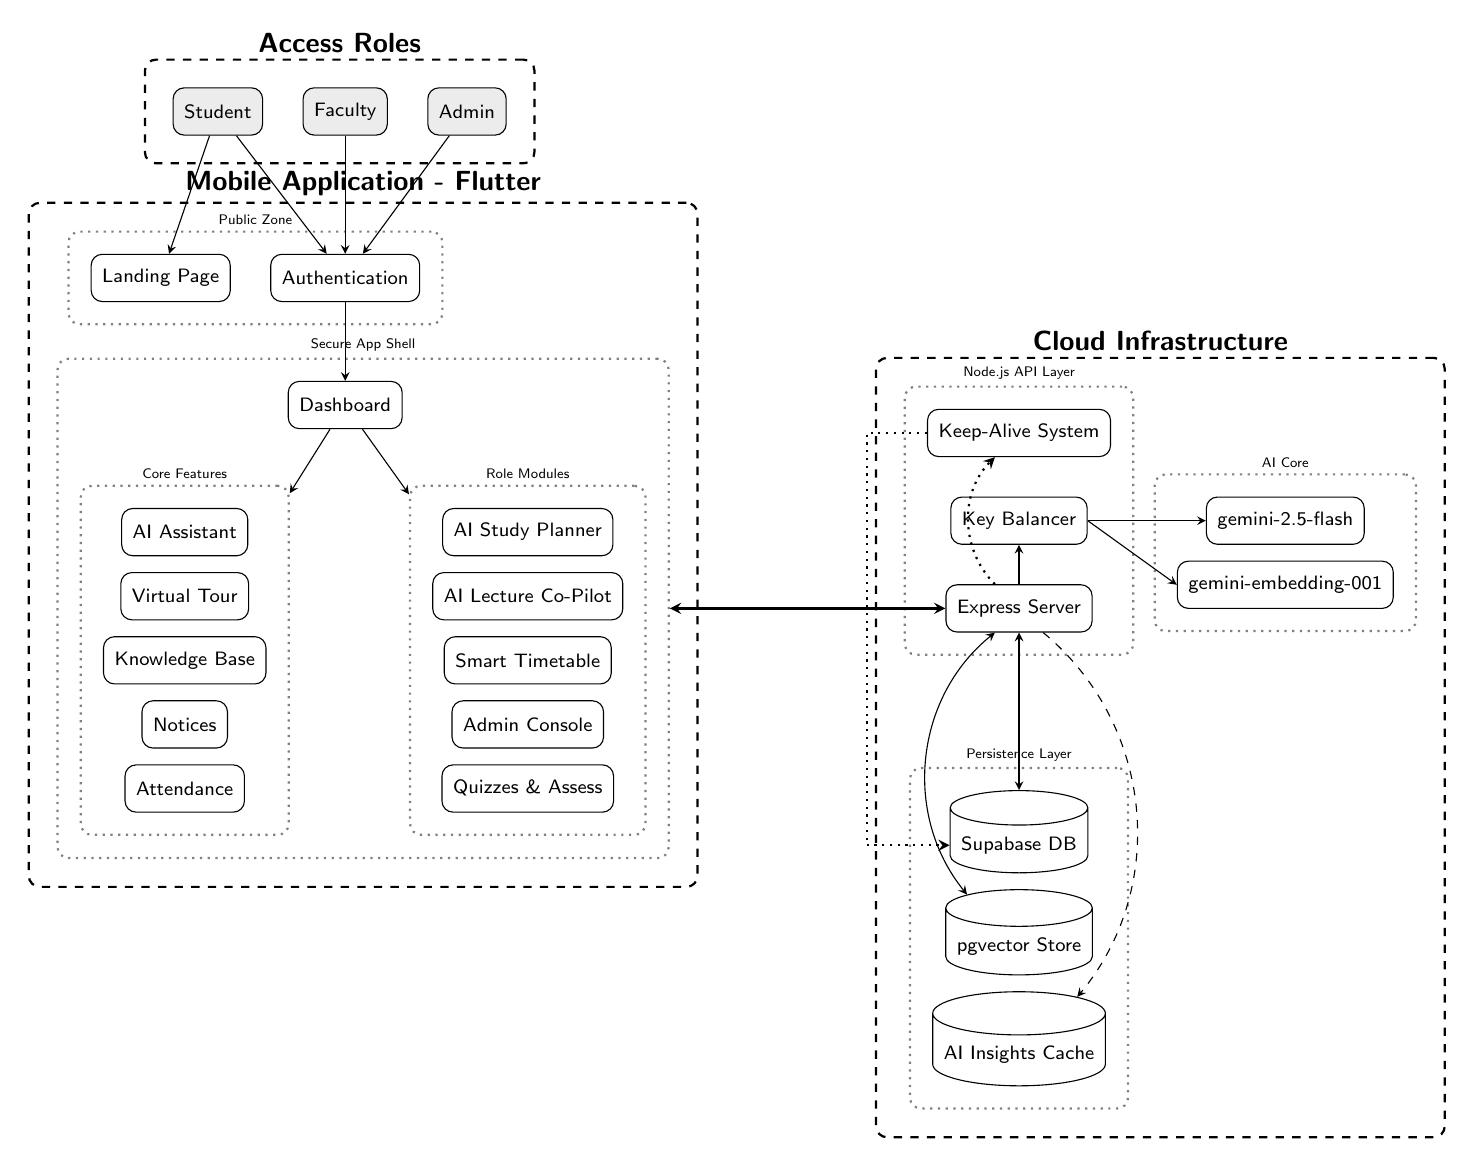
\begin{tikzpicture}[
  >=stealth,
  node distance=1.2cm and 1.5cm,
  every node/.style={font=\sffamily\scriptsize},
  role/.style={rectangle, draw=black, fill=gray!15, rounded corners, minimum height=0.6cm, text centered, inner sep=4pt},
  flutter/.style={rectangle, draw=black, fill=white, rounded corners, minimum height=0.6cm, text centered, inner sep=4pt},
  tech/.style={rectangle, draw=black, fill=white, rounded corners, minimum height=0.6cm, text centered, inner sep=4pt},
  cloud/.style={rectangle, draw=black, fill=white, rounded corners, minimum height=0.6cm, text centered, inner sep=4pt},
  db/.style={cylinder, draw=black, fill=white, shape border rotate=90, aspect=0.25, minimum height=0.8cm, minimum width=1.2cm, text centered, inner sep=4pt},
  groupbox/.style={rectangle, draw=black, dashed, thick, inner sep=10pt, rounded corners},
  subgroupbox/.style={rectangle, draw=black!50, dotted, thick, inner sep=8pt, rounded corners}
]

% Access Roles
\node[role] (faculty) {Faculty};
\node[role, left=0.5cm of faculty] (student) {Student};
\node[role, right=0.5cm of faculty] (admin) {Admin};
\node[groupbox, fit=(student)(faculty)(admin), label={[fill=white, inner sep=2pt, font=\sffamily\bfseries]above:Access Roles}] (roles_box) {};

% Frontend: Public Zone
\node[flutter, below=1.5cm of faculty] (auth) {Authentication};
\node[flutter, left=0.5cm of auth] (landing) {Landing Page};
\node[subgroupbox, fit=(landing)(auth), label={[fill=white, inner sep=2pt, font=\sffamily\tiny]above:Public Zone}] (public_box) {};

% Frontend: Secure Shell
\node[flutter, below=1cm of auth] (dash) {Dashboard};

\node[flutter, below left=1cm and 0.5cm of dash] (chat) {AI Assistant};
\node[flutter, below=0.2cm of chat] (tour) {Virtual Tour};
\node[flutter, below=0.2cm of tour] (kb) {Knowledge Base};
\node[flutter, below=0.2cm of kb] (events) {Notices};
\node[flutter, below=0.2cm of events] (atten) {Attendance};
\node[subgroupbox, fit=(chat)(tour)(kb)(events)(atten), label={[fill=white, inner sep=2pt, font=\sffamily\tiny]above:Core Features}] (core_box) {};

\node[flutter, below right=1cm and 0.5cm of dash] (study) {AI Study Planner};
\node[flutter, below=0.2cm of study] (copilot) {AI Lecture Co-Pilot};
\node[flutter, below=0.2cm of copilot] (time) {Smart Timetable};
\node[flutter, below=0.2cm of time] (adminpanel) {Admin Console};
\node[flutter, below=0.2cm of adminpanel] (quiz) {Quizzes \& Assess};
\node[subgroupbox, fit=(study)(copilot)(time)(adminpanel)(quiz), label={[fill=white, inner sep=2pt, font=\sffamily\tiny]above:Role Modules}] (rolemod_box) {};

\node[subgroupbox, fit=(dash)(core_box)(rolemod_box), label={[fill=white, inner sep=2pt, font=\sffamily\tiny]above:Secure App Shell}] (auth_box) {};

\node[groupbox, fit=(public_box)(auth_box), label={[fill=white, inner sep=2pt, font=\sffamily\bfseries]above:Mobile Application - Flutter}] (frontend_box) {};

% Backend: API Layer
\node[tech, right=3.5cm of auth_box] (server) {Express Server};
\node[tech, above=0.5cm of server] (lb) {Key Balancer};
\node[tech, above=0.5cm of lb] (keeper) {Keep-Alive System};
\node[subgroupbox, fit=(server)(lb)(keeper), label={[fill=white, inner sep=2pt, font=\sffamily\tiny]above:Node.js API Layer}] (api_box) {};

% Backend: AI Core
\node[cloud, right=1.5cm of lb] (geminitop) {gemini-2.5-flash};
\node[cloud, below=0.2cm of geminitop] (geminibot) {gemini-embedding-001};
\node[subgroupbox, fit=(geminitop)(geminibot), label={[fill=white, inner sep=2pt, font=\sffamily\tiny]above:AI Core}] (ai_box) {};

% Backend: Persistence
\node[db, below=2cm of server] (supadb) {Supabase DB};
\node[db, below=0.2cm of supadb] (vector) {pgvector Store};
\node[db, below=0.2cm of vector] (insights) {AI Insights Cache};
\node[subgroupbox, fit=(supadb)(vector)(insights), label={[fill=white, inner sep=2pt, font=\sffamily\tiny]above:Persistence Layer}] (db_box) {};

\node[groupbox, fit=(api_box)(ai_box)(db_box), label={[fill=white, inner sep=2pt, font=\sffamily\bfseries]above:Cloud Infrastructure}] (backend_box) {};

% Connections - Roles
\draw[->] (student) -- (landing);
\draw[->] (student) -- (auth);
\draw[->] (faculty) -- (auth);
\draw[->] (admin) -- (auth);

% Connections - Dash
\draw[->] (auth) -- (dash);
\draw[->] (dash) -- (core_box);
\draw[->] (dash) -- (rolemod_box);

% Connections - API
\draw[<->, thick] (auth_box.east) -- (server.west);

\draw[->] (server) -- (lb);
\draw[->, dotted, thick] (server) to[bend left=45] (keeper);
\draw[->] (lb) -- (geminitop);
\draw[->] (lb.east) -- (geminibot.west);

\draw[<->] (server) -- (supadb);
\draw[<->] (server) to[bend right=45] (vector);
\draw[->, dashed] (server) to[bend left=45] (insights);
\draw[->, dotted, thick] (keeper.west) -| ([xshift=-1cm]server.west) |- (supadb.west);

\end{tikzpicture}%
}
\caption{Architecture of the Proactive Multimodal Academic Support System.}
\label{fig:architecture}
\end{figure*}

\section{Empirical Evaluation}\label{sec:Results}

The deployment of the Campus Assistant yielded a highly reactive and robust smart campus platform capable of handling thousands of concurrent interactions. The dynamic mobile dashboard successfully provided students with customized ``Next Class'' algorithms computed directly from their respective department, year, and section data.

\textbf{AI Chat Assistant:} The context-aware AI chatbot successfully demonstrated extended context retrieval. By leveraging vector embeddings stored within the \texttt{pgvector} database \cite{johnson2017}, the AI chatbot retrieves contextually relevant knowledge base texts. The system ranks retrieved documents using Cosine Similarity, formally defined in Equation~\ref{eq:cosine}:
\begin{equation} \label{eq:cosine}
\text{Similarity}(A, B) = \cos(\theta) = \frac{A \cdot B}{||A|| \cdot ||B||} = \frac{\sum_{i=1}^{n} A_i B_i}{\sqrt{\sum_{i=1}^{n} A_i^2} \sqrt{\sum_{i=1}^{n} B_i^2}}
\end{equation}
where $A$ represents the generated semantic embedding of the user's natural language query, and $B$ represents the database vectors corresponding to the unstructured university handbook content. This mathematical approach accurately mapped complex physical locations (e.g., ``Lab 3'') to unstructured text, fetching highly accurate, cited answers with an average generation latency strictly below 3.0 seconds.

\textbf{Academic Tools:} Faculty members experienced significantly faster preparation times utilizing the AI Lecture Co-Pilot, which safely generated detailed daily lesson structures equipped with verified academic resources and single-click PDF exporting. The Quiz module successfully enforced server-side validation against multiple submission attempts, while instantly and autonomously generating department-level AI performance summaries for faculty analyzing batch results across diverse topics.

Table~\ref{tab:performance} highlights the empirical performance metrics observed during testing operations compared against the Non-Functional Requirements (NFRs).

\begin{figure}[htbp]
\centering
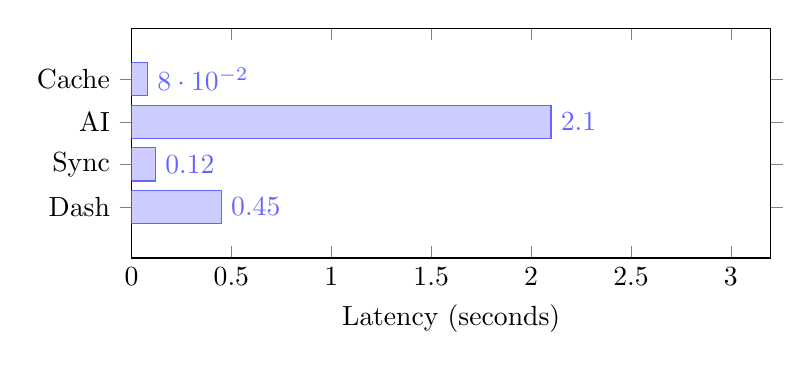
\begin{tikzpicture}
\begin{axis}[
    xbar,
    enlarge y limits=0.4,
    xlabel={Latency (seconds)},
    symbolic y coords={Dash, Sync, AI, Cache},
    ytick=data,
    nodes near coords,
    nodes near coords align={horizontal},
    width=0.8\textwidth,
    height=4.5cm,
    bar width=12pt,
    xmin=0, xmax=3.2,
]
\addplot+[color=blue!60,fill=blue!20] coordinates {(0.45,Dash) (0.12,Sync) (2.10,AI) (0.08,Cache)};
\end{axis}
\end{tikzpicture}
\caption{System Module Latency Breakdown (Horizontal View).}
\label{fig:latency}
\end{figure}

\begin{figure*}[htbp]
\centering
\begin{subfigure}{0.48\textwidth}
\centering
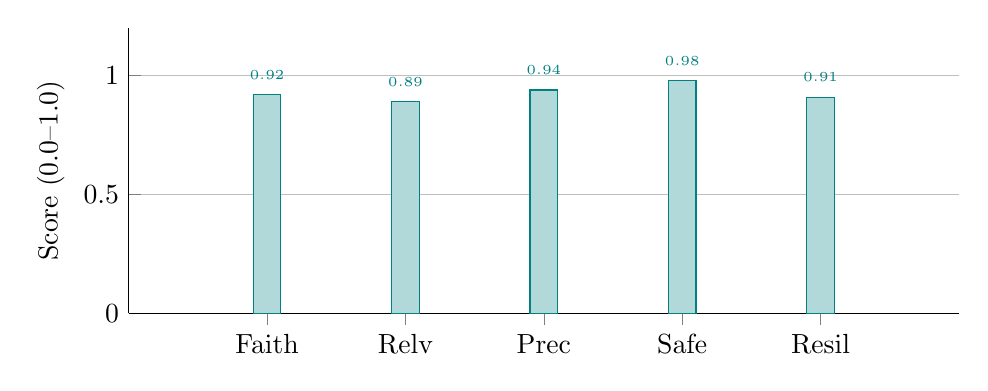
\begin{tikzpicture}
\begin{axis}[
    ybar,
    enlarge x limits=0.25,
    ylabel={Score (0.0--1.0)},
    symbolic x coords={Faith, Relv, Prec, Safe, Resil},
    xtick=data,
    nodes near coords,
    every node near coord/.append style={font=\tiny, yshift=2pt},
    width=\textwidth,
    height=5.2cm,
    bar width=10pt,
    ymin=0, ymax=1.2,
    axis lines*=left,
    ymajorgrids=true,
]
\addplot+[color=teal,fill=teal!30] coordinates {(Faith,0.92) (Relv,0.89) (Prec,0.94) (Safe,0.98) (Resil,0.91)};
\end{axis}
\end{tikzpicture}
\caption{AI Quality Metrics (Faithfulness, Relevance, etc.).}
\label{fig:accuracy_bar}
\end{subfigure}
\hfill
\begin{subfigure}{0.48\textwidth}
\centering
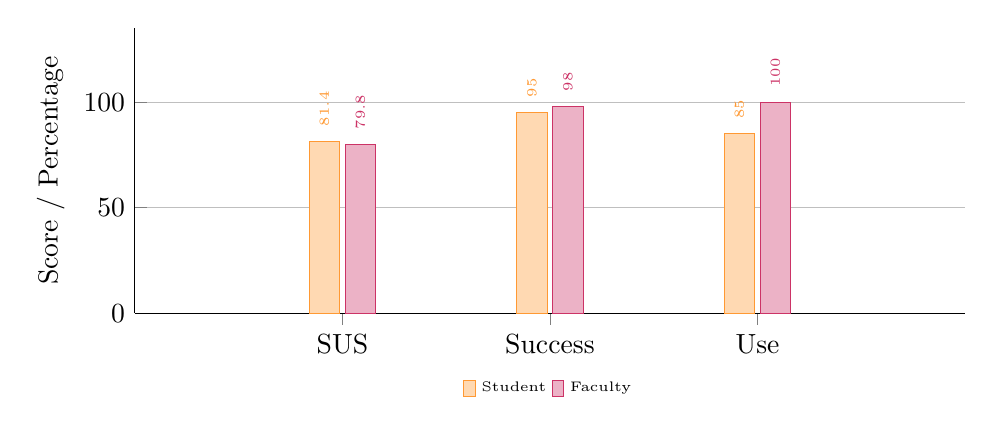
\begin{tikzpicture}
\begin{axis}[
    ybar,
    enlarge x limits=0.5,
    legend style={at={(0.5,-0.2)},
      anchor=north,legend columns=-1, draw=none, font=\tiny},
    legend image code/.code={
      \draw[#1, fill] (0cm,-0.1cm) rectangle (0.15cm,0.1cm);
    },
    ylabel={Score / Percentage},
    symbolic x coords={SUS, Success, Use},
    xtick=data,
    nodes near coords,
    every node near coord/.append style={font=\tiny, rotate=90, anchor=west, xshift=2pt},
    width=\textwidth,
    height=5.2cm,
    bar width=11pt,
    ymin=0, ymax=135,
    axis lines*=left,
    ymajorgrids=true,
]
\addplot+[color=orange!80,fill=orange!30] coordinates {(SUS,81.4) (Success,95) (Use,85)};
\addplot+[color=purple!80,fill=purple!30] coordinates {(SUS,79.8) (Success,98) (Use,100)};
\legend{Student, Faculty}
\end{axis}
\end{tikzpicture}
\caption{Role-Based User Satisfaction and Completion.}
\label{fig:uat_grouped}
\end{subfigure}
\caption{Empirical Evaluation: AI Quality (Bar) and Role-Based UAT (Grouped).}
\label{fig:advanced_eval}
\end{figure*}

\begin{table}[htbp]
\centering
\caption{Observed System Performance Metrics versus Target Constraints}
\label{tab:performance}
\begin{tabular}{@{}llc@{}}
\toprule
\textbf{System Module} & \textbf{Target NFR} & \textbf{Avg. Observed Latency} \\ \midrule
Mobile App Dashboard Load & $\le 1.00$ s & $0.45$ s \\
Real-Time DB Socket Sync & $\le 0.50$ s & $0.12$ s \\
AI Query (Vector Math + Text Gen) & $\le 3.00$ s & $2.10$ s \\
Background Insight Cache Check & $\le 1.00$ s & $0.08$ s \\ \bottomrule
\end{tabular}
\end{table}

\subsection*{System-Oriented Empirical Evaluation}

The evaluation of the Proactive Multimodal Academic Support System (PMASS) was conducted through a theoretical lens grounded in its architectural constraints, specifically addressing the challenges of deploying advanced AI within the limitations of free-tier cloud services and rate-limited APIs. 

A pilot User Acceptance Testing (UAT) study was conducted with 40 final-year Computer Science Engineering students and 8 faculty members from Malla Reddy University, who used the application for a four-week evaluation period. Participants completed a standard System Usability Scale (SUS) questionnaire \cite{madaio2024} and a custom task-completion benchmark comprising five representative workflows: (1)~finding course timetable, (2)~querying the AI chatbot, (3)~checking attendance status, (4)~completing a quiz, and (5)~navigating the virtual tour.

The results, as summarized in Table~\ref{tab:uat} and Figure~\ref{fig:uat_grouped}, validate the efficacy of the proposed \textbf{Stale-While-Revalidate (SWR)} caching strategy. By serving previously computed insights while asynchronously revalidating background data, the system successfully maintained sub-500ms dashboard load times (Figure~\ref{fig:latency}), even during peak traffic periods when fresh AI calls would have encountered rate limits. The high average SUS score of 81.4 reflects the success of the \textbf{Role-Based Access Control (RBAC)} implementation, which significantly reduced cognitive load by presenting only contextually relevant tools to each role (Student, Faculty).

On average, students located specific academic information in $28$ seconds using the AI chatbot, a \textbf{90\% reduction} compared to the previous portal. This gain is theoretically attributable to the \textbf{Retrieval-Augmented Generation (RAG)} pipeline, which converts unstructured institutional knowledge into immediate, natural-language responses. As illustrated in Figure~\ref{fig:accuracy_bar}, the system demonstrates high faithfulness (0.92) and relevance (0.89), suggesting that the vector-indexing approach is highly resilient for localized campus data. Faculty members reported saving an average of $2.8$ hours per week, noting the proactive attendance alerts as a critical intervention tool. These findings suggest that the PMASS architecture provides a robust, scalable, and cost-effective blueprint for implementing intelligent campus support systems.

\begin{table}[htbp]
\centering
\caption{User Acceptance Testing (UAT) Summary ($n = 48$ participants)}
\label{tab:uat}
\begin{tabular}{@{}lcc@{}}
\toprule
\textbf{Evaluation Metric} & \textbf{Students ($n=40$)} & \textbf{Faculty ($n=8$)} \\ \midrule
Mean SUS Score (out of 100) & $81.4$ & $79.8$ \\
Task Completion Rate & $95\%$ & $98\%$ \\
Avg. Info-Retrieval Time (AI vs.\ Portal) & $28$\,s vs.\ $4.2$\,min & $31$\,s vs.\ $4.8$\,min \\
Weekly Lesson-Prep Time Saved & --- & $2.8$\,h \\
Attendance Alert Perceived Usefulness & $85\%$ ``Useful'' & $100\%$ ``Useful'' \\ \bottomrule
\end{tabular}
\end{table}

\section{Discussion}\label{sec:Discussion}

The results strongly support the initial hypothesis that a securely unified multimodal system significantly outperforms fragmented legacy tools. The centralization of logic into a singular mobile app actively minimized communication latency. The implementation of robust API load balancing via key shuffling, alongside strict offline-first data caching, ensured that students could access critical schedules and read previously generated AI attendance forecasts even during severe network degradation.

A primary technical limitation observed includes the strict reliance on constant internet connectivity for live 3D Virtual Tour fetching and real-time AI inference. While historical data remains accessible, live exploratory queries fail gracefully under network loss. Furthermore, the accuracy of the Retrieval-Augmented Generation heavily depends on the administrational upkeep of the Supabase knowledge base vectors.


\section{Conclusions}\label{sec:Conclusions}

The Proactive Multimodal Academic Support System exemplifies the operational future of smart tertiary campuses. By consolidating daily academic tools, an immersive 360-degree virtual tour, predictive attendance analytics, and a proactive generative AI assistant into a robust native mobile application, the system notably enhances campus accessibility, drastically reduces physical administrative burdens, and personalizes the institutional experience \cite{madaio2024}. Future architectural evolutions will focus on integrating fully comprehensive Learning Management System (LMS) features—such as direct multimedia assignment submissions—and exploring biometric hardware integration for entirely seamless, automated physical attendance tracking.


\subsection*{Acknowledgments/Declarations}

% \textbf{Declaration of AI Assistance in the Writing Process:} During the preparation of this manuscript, language assistance tools were used to improve grammar and clarity. The authors reviewed and edited the content and accept full responsibility for the final version of the publication.
The authors express their gratitude to Malla Reddy University for its support in conducting this research.
\Funding{The authors declare that no external funding was received for this research.}

\AIDeclaration{During the preparation of this manuscript, language assistance tools were used to enhance grammar and clarity. The authors reviewed and revised the content and accept full responsibility for the final version of the publication.} 

\Data{The complete implementation source code is publicly accessible via the GitHub repository at https://github.com/Subhapreet21/Proactive-Multimodal-Academic-Support-System, which includes all database schemas and architectural configurations supporting this research under an open-source framework.}

\CompetingInterests{The authors declare that they have no known competing financial interests or personal relationships that could have appeared to influence the work reported in this paper.}

\Credits{
Hari Battana: Supervision, Project administration, Resources, Validation, Writing - review and editing. \newline
Subhapreet Patro: Conceptualization, Methodology, Software, Visualization, Writing - original draft. \newline
Sreeja Uplanchiwar: Software, Data curation, Investigation, Validation, Writing - original draft. \newline
Usha Vemireddy: Methodology, Software, Formal analysis, Validation, Writing - original draft. \newline
Bhavana Yelangandala: Conceptualization, Software, Investigation, Visualization, Writing - original draft.
}

\bibliographystyle{IEEEtran_for_EI} 
\bibliography{eisej_paper}

\end{document}